\documentclass[a4paper, 11pt]{article}

\title{MPFU channel phase dependence on the amplitude}
\author{Gianluca Marcozzi}
\date{2025-01}

\usepackage{amsmath}
\usepackage{graphicx}
\usepackage[style=numeric-comp, sorting=none, backend=biber]{biblatex}
% \addbibresource{reportZePSI_01.bib}

\begin{document}
	\maketitle
	\section*{Materials and methods}
	To calibrate the phase of the microwave pulses for varying MPFU amplitude the spin echo signal from a coal standard is monitored as a function of the MPFU amplitude. The sequence used is $\beta/2$-$\tau$-$\beta$-$\tau$-echo. To avoid an overlap with the ringdown, $\tau$ is set to $500\;\text{ns}$. The pulses are generated from the $+y$-channel of the MPFU. The lengths of the $\pi/2$- and $\pi$-pulses are $6\;\text{ns}$ and $12\;\text{ns}$ respectively. At the attenuation value of $0\;\text{dB}$ used in the experiment, these values ensure that $\beta = \pi$ at the maximum value of MPFU amplitude (as seen from Rabi nutations, not shown here). Theoretically, the phase of the echo is independent of the turning angle. Any phase deviation is due to spectrometer components and has to be calibrated and corrected (hence motivating this experiment).\\
	The amplitude of the MPFU channel is stepped linearly from $78.0\%$ to $83.0\%$, for a total of $51$ measurements. Note that a linear increase in the amplitude of the MPFU channel does not correspond to a linear increase of the $B_1$ intensity. A previous calibration of the $B_1$ intensity as a function MPFU channel amplitude was carried out via Rabi nutations experiments (not shown here).\\
	The experiment is conducted at $T = 150\;\text{K}$.
	
	\section*{Experimental results}
	The acquired echo are shown in Fig. \ref{fig:exampleEcho}. All the data can be found in the appendix. \\
	One can see that for this amplitude value the echo is positive in the $0^o$ channel and almost zero in the $90^o$ channel.
	\begin{figure}
		\centering
		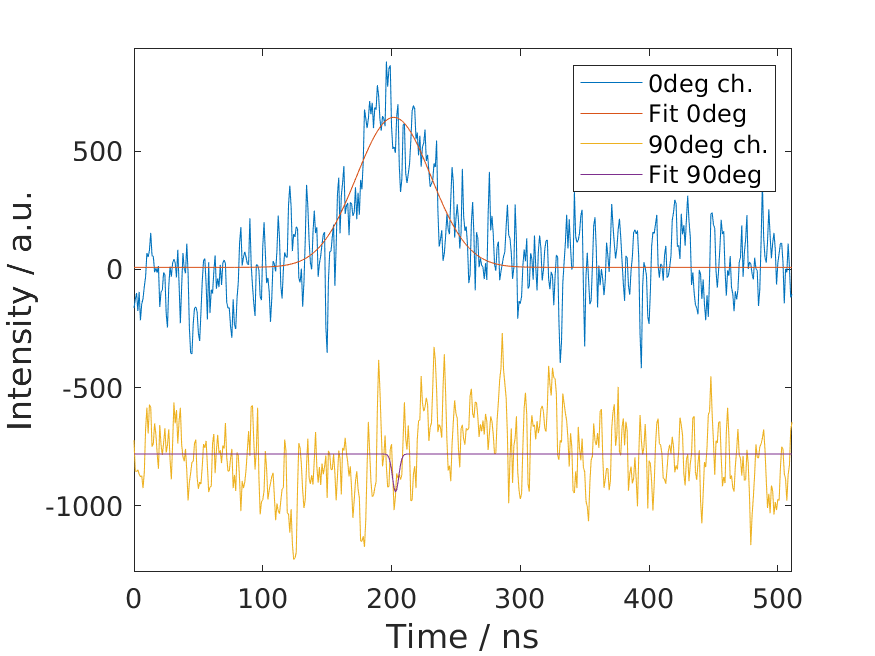
\includegraphics[width=0.95\textwidth]{../../images/misc-E-001_exampleEcho}
		\caption{Echo obtained for a MPFU amplitude value of $79.0\%$ with overlaying gaussian fit.}
		\label{fig:exampleEcho}
	\end{figure}
	
	\section*{Data analysis}
	All the data was fitted with a gaussian function in an automated fashion. The phase $\phi$ and the total intensity $\rho$ were determined as follows:
	\begin{equation}
		\phi = \tan{\left(\frac{B}{A}\right)},
		\quad
		\rho = \sqrt{A^2 + B^2},
	\end{equation}
	where $A$ and $B$ are the values of the integral of the $0^o$ and the $90^o$ channel, respectively. The results obtained are shown in Fig. \ref{fig:phaseAndIntensity_vs_mpfuAmp}. Even with such noise in the phase determination for MPFU amplitudes smaller than $80\%$, a sigmoidal trend is visible.
	\begin{figure}
		\centering
		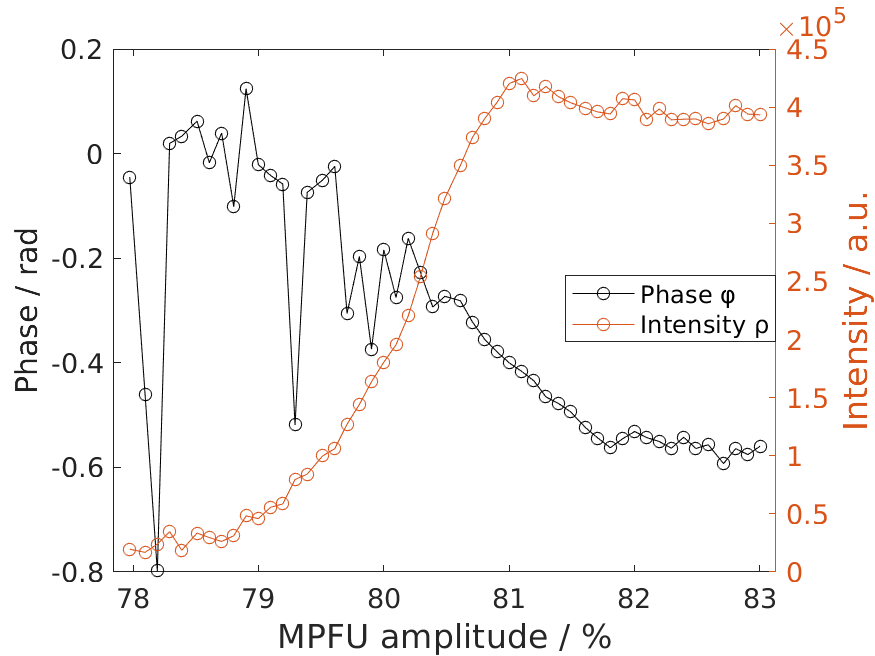
\includegraphics[width=0.95\textwidth]{../../images/misc-E-001_phaseAndIntensity_vs_mpfuAmp}
		\caption{Phase $\phi$ and total intensity $\rho$ as a function of MPFU amplitude.}
		\label{fig:phaseAndIntensity_vs_mpfuAmp}
	\end{figure}
	
	\section*{Outlook}
	In this experiment, the pulse lengths have been mantained constant. To improve the signal to noise for values of MPFU amplitude smaller than $80\%$, an experiment where longer pulses are used for smaller values of MPFU amplitude must be carried out.
	
\end{document}
